\documentclass[12pt]{article}

\usepackage[ngerman]{babel}
\usepackage[babel,german=swiss]{csquotes} % Schweizer

\usepackage{natbib}

\usepackage{graphicx}
\usepackage{amsmath, amsthm, amssymb}
\usepackage{mathtools}
\usepackage{array}
\usepackage{fancyhdr}
\usepackage{xcolor}
\usepackage{wrapfig}
\usepackage{tabularx}
\usepackage{float}
\usepackage{parskip}

\usepackage{fontspec,xltxtra,xunicode}
\defaultfontfeatures{Mapping=tex-text}
\setromanfont[Mapping=tex-text]{Calibri}
\setsansfont[Scale=MatchLowercase,Mapping=tex-text]{Gill Sans}
\setmonofont[Scale=MatchLowercase]{Andale Mono}
\linespread{1.2}

% Definition der Seite
\usepackage[paper=a4paper]{geometry} 

% Header Layout
\pagestyle{fancy}
\fancyhf{}
\fancyhead[L]{Projektarbeit: Doppelt inverses Pendel}
\fancyfoot[C]{\thepage}
\renewcommand{\headrulewidth}{0.1pt}
\renewcommand{\footrulewidth}{0.0pt}

\setlength{\headheight}{15pt}
\setcounter{secnumdepth}{4}
\setcounter{tocdepth}{4}

% PDF Einstellungen
\usepackage[draft=false, debug=false]{hyperref}
\hypersetup{
	pdfauthor={Michael Höhn, Stefan Hauenstein},
	pdftitle={Projektarbeit: Doppelt inverses Pendel},
	bookmarks,
	colorlinks,%
    citecolor=black,%
    filecolor=black,%
    linkcolor=black,%
    urlcolor=black
}

% Paragraph
\setlength\parindent{0pt} 
\setlength{\parskip}{0.75em}

% set graphics
\graphicspath{{./images/},{./appendix/}}
\DeclareGraphicsExtensions{.png, .jpg, .pdf}

% set equation numbering
\numberwithin{equation}{subsection}

\makeatletter
\renewcommand\paragraph{\@startsection{paragraph}{4}{\z@}%
  {-3.25ex\@plus -1ex \@minus -.2ex}%
  {1.5ex \@plus .2ex}%
  {\normalfont\normalsize\bfseries}}
  
% No dots in TOC
\renewcommand{\@dotsep}{10000}
\makeatother

\title{\vspace{-1cm}\linespread{1}\begin{flushleft}\normalsize{Zürcher Hochschule für Angewandte Wissenschaften\\Studiengang Informatik\\}\end{flushleft}\vspace{2cm}\Large{Projektarbeit: Doppelt inverses Pendel}\\\vspace{2cm} 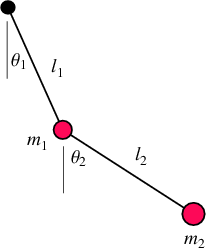
\includegraphics[scale=1]{title.png} \\ \tiny{Bild: Wolfram Research}}

\author{Michael Höhn\\\href{mailto:hoehnmic@students.zhaw.ch}{hoehnmic@students.zhaw.ch} \and Stefan Hauenstein\\\href{mailto:hauenste@students.zhaw.ch}{hauenste@students.zhaw.ch}}

\date{\today}

% Titelseite
\begin{document}
\maketitle\thispagestyle{empty}
\newpage

% Inhaltsverzeichnis
\tableofcontents


% Projektbeschreibung
\newpage
\section{Projektbeschreibung}
\subsection{Danksagung}
Wir möchten an dieser Stelle Herrn Georg Brügger und Herrn Lukas Eppler danken, ohne ihre wertvolle Unterstützung und Anregungen wäre dieses Software Projekt nur schwer umsetzbar gewesen.

\subsection{Aufgabenstellung durch den Experten}
Das Schwingverhalten eines idealen „Doppelt inversen Pendels“ soll untersucht und durch geeignete physikalische und mathematische Beziehungen nachgebildet werden. Physikalische Effekte wie Reibung und Luftwiderstand werden vernachlässigt, Abmessungen und Materialien müssen als Eingabegrössen variabel gestaltet werden.

Der Vorgang wird in „Echtzeit“ am Bildschirm des Computers graphisch dargestellt visualisiert.

Zusätzliche Angaben des Verhaltens können auf der gleichen Seite eingeblendet werden.

\subsection{Motivation}
Physikalische Eigenschaften mit einer objektorientierten Programmiersprache umzusetzen, reizte uns schon immer. Die  Aufgabenstellung ermöglichte uns, das theoretisch Gelernte aus dem Studienfach Numerik in Verbindung mit physikalischen Grundlagen in einer praktischen Anwendung umzusetzen. Auch ermöglichte es die algebraischen Zusammenhänge aus vergangenen Vorlesungen besser zu verstehen und Lücken aufzufüllen.

\subsection{Beteiligte Personen}
\begin{tabularx}{\textwidth}{|X|X|}
	\hline
	\textbf{Funktion} & \textbf{Name} \\
	\hline
	Projekt Team      & Stefan Hauenstein \\
	                  & Michael Höhn \\
	\hline
	Experte           & Georg Brügger\\
	\hline
	Scrum Master      & Lukas Eppler\\
	\hline
\end{tabularx}


% Anforderungsanalyse
\newpage
\section{Anforderungsanalyse}
\subsection{Zielbestimmung}
Es soll ein Programm entwickelt werden, das die physikalischen und chaotischen Eigenschaften des Doppelt inversen Pendels grafisch darstellt.

Die einzelnen Segmente des Pendels sollen durch Benutzereingaben über Tastatur und/oder Maus einstellbar sein.

\subsection{Rahmenbedingungen und Einschränkungen}
\begin{itemize}
	\item Die Umgebung des Doppelpendels soll als ideal gelten.
	\item Als Ausgangsmaterial des Pendels wird Aluminium definiert (Dichte $2,7 [g/cm^3]$)
	\item Die Gravitation wird mit $9.81 [m/s^2]$ definiert
	\item Wegen der chaotischen Eigenschaft des Pendels können keine aussagekräftigen Tests implementiert werden.
\end{itemize}

\subsection{Produktfunktionen}
\begin{itemize}
	\item Der Benutzer kann eine Konfiguration als XML-File mit der Erweiterung IDP einlesen.
	\item Der Benutzer kann die einzelnen Glieder des Pendels mit der Maus positionieren.
	\item Während das Pendel in Bewegung ist, werden Winkel und Geschwindigkeit angezeigt.
	\item Der Benutzer kann den Ablauf starten, jederzeit stoppen und zurückstellen.
\end{itemize}


% Umsetzung
\newpage
\section{Umsetzung}

\subsection{Projektplanung}
Um das Softwareprojekt und die einzelnen Iterationen planen und verwalten zu können, wurde Pivotaltracker \citep{pivotal} von Pivotal Labs eingesetzt. Die einzelnen Tasks der Projektplanung können unter \citep{hoehnHauenstein} nachgeschlagen werden.

\subsection{Iterationsplan}
\newcolumntype{L}{>{\raggedright\arraybackslash}X}
\begin{tabularx}{\textwidth}{|l|l|L|}
	\hline
	\textbf{Iteration} & \textbf{Termin}     & \textbf{Story}\\
	\hline
	1                  & Mi 04.04.2012       & \begin{itemize}
													\item Evaluierung der Programmiersprache
													\item Physikalische Eigenschaften des Doppelpendels verstehen
													\item Gleichungssystem aufstellen
											 \end{itemize}\\
	\hline
	2                  & Fr 27.04.2012       & \begin{itemize}
													\item Grafische Benutzeroberfläche
													\item Programmierung des ersten Pendels
													\item Programmierung des zweiten Pendels
													\item Runge Kutta definieren
										   	 \end{itemize}\\
	\hline
	3                  & Mi 23.05.2012       & \begin{itemize}
													\item Pendel einstellen
													\item Projektdokumentation
											 \end{itemize}\\
	\hline
	4                  & SA 16.06.2012       & \begin{itemize}
													\item Projektdokumentation
													\item Präsentation
											 \end{itemize}\\
	\hline
\end{tabularx}

\subsection{Programmiersprache}
Das Programm wird mittels der objektorientierten Programmiersprache ActionScript 3 (AS3) und dem Adobe Flex SDK Framework \citep{flex} implementiert. Es ist dank dem Adobe Flashplayer auf fast jedem Betriebssystem und Browser lauffähig.

Eine Implementierung des Doppelpendels mittels AS3 und dem Flex SDK ist empfehlenswert, da das Flex Framework speziell für grafische Applikationen mit Animationen ausgelegt ist und es dadurch zu einer grossen Zeiteinsparung bei der Entwicklung kommt.

\subsection{Grafische Oberfläche}
Die grafische Oberfläche wird als skalierbares Modell aufgebaut. Der Vorteil in diesem Aufbau besteht darin, dass die Applikation auf jeder Bildschirmauflösung optimal dargestellt wird. Die Grösse der Pendelsimulation passt sich anhand der Fenstergrösse automatisch an.

\begin{figure}[H]
	\centering
	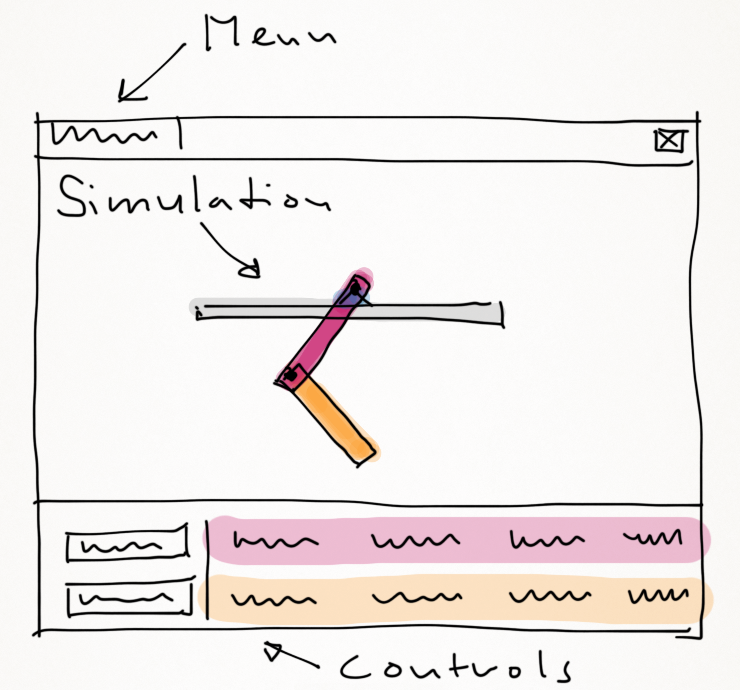
\includegraphics[width=\textwidth]{software_draft.png}
	\caption{Entwurf grafische Oberfläche}
	\label{fig:gui:draft}
\end{figure}


% Physikalische und mathematische Zusammenhänge
\newpage
\section{Physikalische und mathematische Zusammenhänge}

\subsection{Funktionsprinzip Doppelpendel}
\begin{figure}[H]
	\centering
	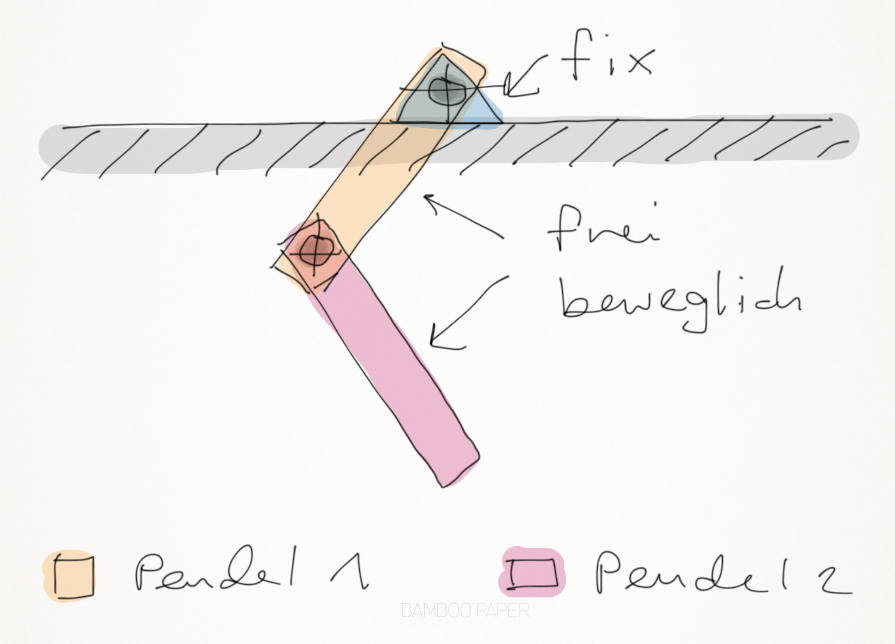
\includegraphics[width=\textwidth]{function.png}
	\caption{Funktionsweise des Doppelpendels}
	\label{fig:function}
\end{figure}

\subsection{Physikalische Eigenschaften}
Um die Gleichungen des Ausgangsproblems zu definieren, muss man sich erst mit den physikalischen Eigenschaften eines Pendels beschäftigen. Kräfte, welche aus der Bewegung entstehen, kombinieren sich mit Statischen. Kräfte des ersten Pendels beeinflussen die des zweiten. Im Folgenden werden die Kinematik und die Kräfte des Doppelpendels zum gesuchten Ausgangsproblem kombiniert.

Auf Basis der Webseiten \citep{neumann04}, \citep{kramann11} und \citep{weissstein07} konnten die Kinematik und Kräfte des Doppelpendels zum Ausgangsproblem kombiniert werden. 

\subsubsection{Kinematik des Doppelpendels}
\begin{figure}[H]
	\begin{minipage}[!b]{0.4\textwidth}
		\centering
		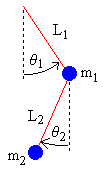
\includegraphics[scale=1]{dbl_pendulum.png}
		\caption[Doppelpendel]{Doppelpendel \citep{neumann04}}
		\label{fig:energy}
	\end{minipage}
	\begin{minipage}[!t]{\textwidth}
		\vspace{0pt}\raggedright
		$x$ = Horizontale Position des Massenschwerpunkts\\
		$y$ = Vertikale Position des Massenschwerpunkts\\
		$\theta$ = Winkel\\
		$L$ = Pendellänge
	\end{minipage}
\end{figure}

Ausgangslage für die Berechnung ist das obere Pendel. Das erste Pendel $P_1$ wird definiert mit $x_1$ und $y_1$. Äquivalent dazu wird das zweite Pendel $P_2$ definiert mit $x_2$ und $y_2$.

Als erstes werden die trigonometrischen Gleichungen aufgestellt:
\begin{equation} \label{eq:energy:1_1}
	x_1 = L_1\sin\theta_1
\end{equation}
\begin{equation} \label{eq:energy:1_2}
	y_1 = -L_1\cos\theta_1
\end{equation}

\begin{equation} \label{eq:energy:2_1}
	x_2 = x_1 + L_2\sin\theta_2
\end{equation}
\begin{equation} \label{eq:energy:2_2}
	y_2 = y_1 - L_2\cos\theta_2
\end{equation}
\
\\
Danach wird aus den Gleichungen (\ref{eq:energy:1_1} - \ref{eq:energy:2_2}) die erste und zweite Ableitung gebildet.

Erste Ableitung (Geschwindigkeit):
\begin{equation} \label{eq:velocity:1_1}
	x_1' = \theta_1' L_1\cos\theta_1
\end{equation}
\begin{equation} \label{eq:velocity:1_2}
	y_1' = \theta_1' L_1\sin\theta_1
\end{equation}

\begin{equation} \label{eq:velocity:2_1}
	x_2' = x_1' + \theta_2' L_2\cos\theta_2
\end{equation}
\begin{equation} \label{eq:velocity:2_2}
	y_2' = y_1' + \theta_2' L_2\sin\theta_2
\end{equation}
\
\\
Zweite Ableitung (Beschleunigung):
\begin{equation} \label{eq:acceleration:1_1}
	x_1'' = -{\theta_1'}^2 L_1 \sin\theta_1 + \theta_1'' L_1 \cos\theta_1
\end{equation}
\begin{equation} \label{eq:acceleration:1_2}
	y_1'' = {\theta_1'}^2 L_1 \cos\theta_1 + \theta_1'' L_1 \sin\theta_1
\end{equation}

\begin{equation} \label{eq:acceleration:2_1}
	x_2'' = x_1'' - {\theta_2'}^2 L_2\sin\theta_2 + \theta_2'' L_2 \cos\theta_2
\end{equation}
\begin{equation} \label{eq:acceleration:2_2}
	y_2'' = y_1'' + {\theta_2'}^2 L_2\cos\theta_2 + \theta_2'' L_2 \sin\theta_2
\end{equation}
\clearpage

\subsubsection{Kräfte im Doppelpendel}
Die Kräfte werden pro Pendel berechnet und in einzelne Gleichungen gesetzt. Auf Grundlage des zweiten newtonschen Gesetzes $(F = m \cdot a)$ können folgende Gleichungen für das Doppelpendel erstellt werden:

\paragraph{Oberes Pendel}
\begin{figure}[H]
	\begin{minipage}[!b]{0.5\textwidth}
		\centering
		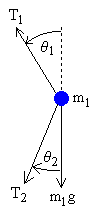
\includegraphics[scale=1]{dbl_pendulum_m1.png}
		\caption[Kräfte im oberen Pendel]{Kräfte im oberen Pendel \citep{neumann04}}
		\label{fig:force_1}
	\end{minipage}
	\begin{minipage}[!t]{\textwidth}
		\vspace{0pt}\raggedright
		$T_1$ = Kraft im oberen Pendel\\
		$m_1$ = Masse des oberen Pendels\\
		$g$ = Gravitationskonstante
	\end{minipage}
\end{figure}

Anhand von \autoref{fig:force_1} können die folgenden Gleichungen aufgestellt werden.
\begin{equation} \label{eq:force:1_1}
	m_1 x_1'' = -T_1\sin\theta_1 + T_2\sin\theta_2
\end{equation}
\begin{equation} \label{eq:force:1_2}
	m_1 y_1'' = T_1\cos\theta_1 + T_1\cos\theta_2 - m_1 g
\end{equation}
\clearpage

\paragraph{Unteres Pendel}
\begin{figure}[H]
	\begin{minipage}[!b]{0.5\textwidth}
		\centering
		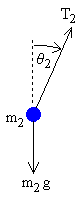
\includegraphics[scale=1]{dbl_pendulum_m2.png}
		\caption[Kräfte im unteren Pendel]{Kräfte im unteren Pendel \citep{neumann04}}
		\label{fig:force_2}
	\end{minipage}
	\begin{minipage}[!t]{\textwidth}
		\vspace{0pt}\raggedright
		$T_2$ = Kraft im unteren Pendel\\
		$m_2$ = Masse des unteren Pendels\\
		$g$ = Gravitationskonstante
	\end{minipage}
\end{figure}

Anhand von \autoref{fig:force_2} können die folgenden Gleichungen aufgestellt werden.
\begin{equation} \label{eq:force:2_1}
	m_2 x_2'' = -T_2\sin\theta_2
\end{equation}
\begin{equation} \label{eq:force:2_2}
	m_2 y_2'' = T_2\cos\theta_2 - m_2 g
\end{equation}

\subsubsection{Umformen der Gleichungen}
Um zu der endgültigen differenziellen Gleichung für die Berechnung zu gelangen, müssen die einzelnen Gleichungen algebraisch umgeformt werden. Die Kräftegleichungen (\ref{eq:force:2_1}) und (\ref{eq:force:2_2}) werden nach $T_2\sin\theta_2$ bzw. nach $T_2\cos\theta_2$ aufgelöst und in die Gleichungen (\ref{eq:force:1_1}) und (\ref{eq:force:1_2}) eingesetzt.
\begin{equation} \label{eq:dForce:1}
	m_1 x_1'' = -T_1\sin\theta_1 - m_2 x_2''
\end{equation}
\begin{equation} \label{eq:dForce:2}
	m_1 y_1'' = T_1\cos\theta_1 -m_2 y_2'' - m_2 g - m_1 g
\end{equation}

Gleichung (\ref{eq:dForce:1}) wird mit $\cos\theta_1$ und Gleichung (\ref{eq:dForce:2}) mit $\sin\theta_1$ erweitert und nach $T_1\sin\theta_1\cos\theta_1$ aufgelöst.
\begin{equation} \label{eq:thetaForce:1_1}
	T_1\sin\theta_1\cos\theta_1 = -\cos\theta_1(m_1 x_1'' + m_2 x_2'')
\end{equation}
\begin{equation} \label{eq:thetaForce:1_2}
	T_1\sin\theta_1\cos\theta_1 = \sin\theta_1(m_1 y_1'' + m_2 y_2'' + m_2 g + m_1 g)
\end{equation}
\
\\
Daraus ergibt sich der erste Teil der Bewegungsgleichung.
\begin{equation} \label{eq:motion:1}
	\sin\theta_1(m_1 y_1'' + m_2 y_2'' + m_2 g + m_1 g) = -\cos\theta_1(m_1 x_1'' + m_2 x_2'')
\end{equation}
\
\\
Um den zweiten Teil der Gleichung zu erhalten, wird die Gleichung (\ref{eq:force:2_1}) mit $\cos\theta_2$ und die (\ref{eq:force:2_2}) mit $\sin\theta_2$ erweitert.
\begin{equation} \label{eq:thetaForce:2_1}
	T_2\sin\theta_2\cos\theta_2 = -\cos\theta_2(m_2 x_2'')
\end{equation}
\begin{equation} \label{eq:thetaForce:2_2}
	T_2\sin\theta_2\cos\theta_2 = \sin\theta_2(m_2 y_2'' + m_2 g)
\end{equation}
\
\\
Der zweite Teil der Gleichung ergibt somit
\begin{equation} \label{eq:motion:2}
	\sin\theta_2(m_2 y_2'' + m_2 g) = -\cos\theta_2(m_2 x_2'')
\end{equation}
\
\\
$x_2''$, $x_2''$, $y_1''$ und $y_2''$ werden durch die Gleichungen (\ref{eq:acceleration:1_1} – \ref{eq:acceleration:2_2}) ersetzt und mit Hilfe des Lagrange-Formalismus nach $\theta_1''$ und $\theta_2''$ aufgelöst.

Die endgültige Bewegungsgleichung für das Doppelpendel lautet somit:
\begin{equation} \label{eq:final:1}
	\theta_1'' = \frac{-g(2m_1+m_2)\sin\theta_1 - m_2 g \sin(\theta_1 - 2\theta_2) -2\sin(\theta_1 - \theta_2)m_2({\theta_2'}^2 L_2 + {\theta_1'}^2 L_1\cos(\theta_1 - \theta_2))}
	{L_1(2m_1 + m_2 - m_2 \cos(2\theta_1 - 2\theta_2))}
\end{equation}

\begin{equation} \label{eq:final:2}
	\theta_2'' = \frac{2\sin(\theta_1 - \theta_2)({\theta_1'}^2 L_1(m_1 + m_2) + g(m_1 + m_2)\cos\theta_1 + {\theta_2'}^2 L_2 m_2 \cos(\theta_1 - \theta_2))}
	{L_2 (2m_1 + m_2 - m_2 \cos(2 \theta_1 - 2\theta_2))}
\end{equation}

% Numerisches Verfahren
\newpage
\section{Numerisches Verfahren}
Um den Fehler der numerischen Lösung pro Berechnungsschritt auf möglichst lange Zeit klein zu halten, wird das numerische Verfahren von Runge-Kutta in der 4. Ordnung verwendet. Der Rechenaufwand für dieses Verfahren ist höher als bei anderen Verfahren wie z.B. dem Euler-Verfahren. Seine Genauigkeit auf grosse Zeitintervalle gleichen diesen Mehraufwand jedoch wieder aus.

\subsection{Runge-Kutta Verfahren 4. Ordnung (RK4)}
Das klassische Runge-Kutta-Verfahren (nach Carl Runge und Martin Wilhelm Kutta) ist ein spezielles explizites 4-stufiges Verfahren zur numerischen Lösung von Anfangswertproblemen. Runge hat als erster (1895) ein mehrstufiges Verfahren angegeben und Kutta (1905) die allgemeine Form expliziter s-stufiger Verfahren definiert.

Das klassische Runge-Kutta-Verfahren verwendet den Ansatz Ableitungen durch Differenzenquotienten zu approximieren. Die dabei bei nichtlinearen Funktionen notwendigerweise auftretenden Fehler können durch geeignete Kombinationen verschiedener Differenzenquotienten reduziert werden. Das RK4 verfahren ist eine solche Kombination, die Diskretisierungsfehler bis zur dritten Ableitung kompensiert.

\begin{align} \label{algo:rk}
	y(t)' &= f(t,y(t)) \quad \text{mit} \quad y(0) = y_0 \nonumber\\
	\nonumber\\
	y^{k+1} &= y^k + h \left(\frac{1}{6}k_1 + \frac{2}{6}k_2 + \frac{2}{6}k_3 + \frac{1}{6}k_4 \right)\\
	\nonumber\\
	\text{mit} \quad k_1 &= f(t_k, y^k) \nonumber\\
	k_2 &= f\left(t_k + \frac{h}{2}, y^k + \frac{h}{2}k_1 \right) \nonumber\\
	k_3 &= f\left(t_k + \frac{h}{2}, y^k + \frac{h}{2}k_2 \right) \nonumber\\
	k_4 &= f\left(t_k + h, y^k + h k_3 \right)\nonumber
\end{align}

\subsection{Differentialgleichung für Runge-Kutta}
Die Bewegungsgleichung (\ref{eq:final:1} und \ref{eq:final:2}) lässt sich noch nicht mittels des Runge-Kutta Algorithmus numerisch annähern. Um dies zu ermöglichen, muss bedacht werden, dass die erste Ableitung von $\theta$ die Winkelgeschwindigkeit $\omega$ ist.

Daraus ergibt sich:
\begin{equation*}
	\theta_1' = \omega_1 \quad \text{und} \quad \theta_2' = \omega_2
\end{equation*}
\
\\
damit erhält man für den Runge-Kutta Algorithmus (\ref{algo:rk}) folgende Schlussgleichungen:
\begin{equation} \label{eq:rk:1}
	\theta_1' = \omega_1
\end{equation}
\begin{equation} \label{eq:rk:2}
	\theta_2' = \omega_2
\end{equation}

\begin{equation} \label{eq:rk:3}
	\omega_1' = \frac{-g(2m_1+m_2)\sin\theta_1 - m_2 g \sin(\theta_1 - 2\theta_2) -2\sin(\theta_1 - \theta_2)m_2(\omega_2^2 L_2 + \omega_1^2 L_1\cos(\theta_1 - \theta_2))}
	{L_1(2m_1 + m_2 - m_2 \cos(2\theta_1 - 2\theta_2))}
\end{equation}

\begin{equation} \label{eq:rk:4}
	\omega_2' = \frac{2\sin(\theta_1 - \theta_2)(\omega_1^2 L_1(m_1 + m_2) + g(m_1 + m_2)\cos\theta_1 + \omega_2^2 L_2 m_2 \cos(\theta_1 - \theta_2))}
	{L_2 (2m_1 + m_2 - m_2 \cos(2 \theta_1 - 2\theta_2))}
\end{equation}


% Software
\newpage
\section{Software}
\subsection{Verwendete Technologien}
\subsubsection{Flash Development Tool (FDT)}
Als Entwicklungsumgebung wird FDT \citep{fdt} eingesetzt. FDT stellt für die Entwicklung von AS3 und Flex-Projekten nützliche Funktionen wie Fehlererkennung, Debugger und Autocomplete zur Verfügung.

\subsubsection{Versionskontrolle}
Die Versionskontrolle des Quellcodes wurde mit git \citep{git} umgesetzt. Das Git repository des Doppelt inversen Pendels ist auf GitHub \citep{github} verfügbar. Im Git repository befindet sich auch die Dokumentation und eine Kopie der GNU Public License, unter der diese Software veröffentlicht ist.

\subsection{Aufbau}
Die Klasse \textit{Main} initialisiert die Applikation und platziert sie auf der \textit{Stage} (Hauptcontainer des GUIs), auf die sie durch die Vererbung der AS3 Klasse \textit{Sprite} zugriff hat. Über die \textit{Main} Klasse wird die Hauptklasse \textit{Doppelpendel} instanziert und gestartet. 

Die Sprite-Klasse ist ein AS3-Grundbaustein der Anzeigeliste: ein Knoten der Anzeigeliste, der Grafiken anzeigen und auch untergeordnete Objekte enthalten kann.

\begin{figure}[H]
	\centering
	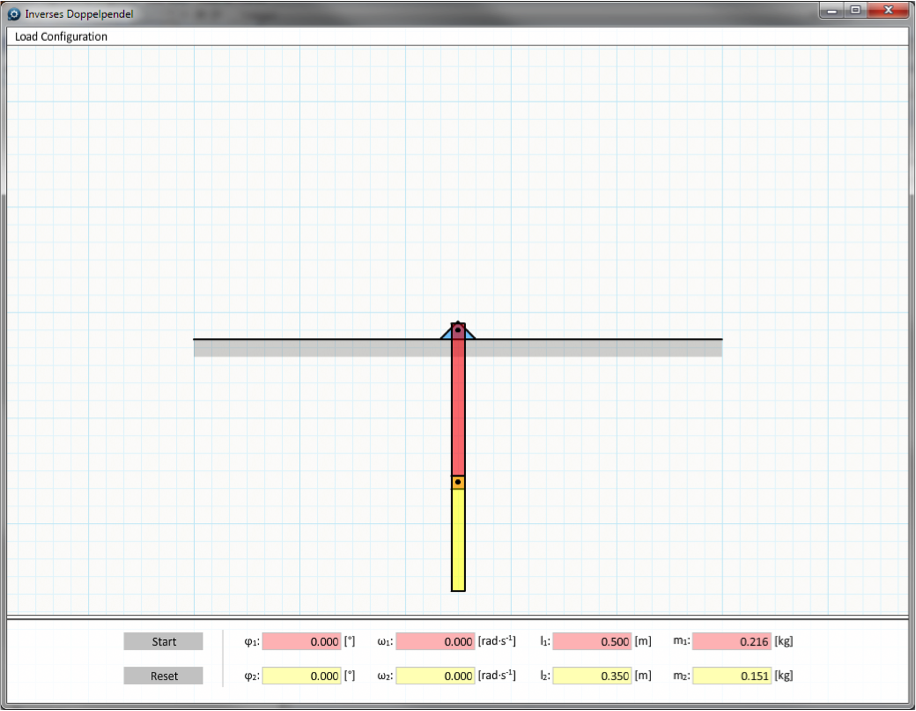
\includegraphics[width=\textwidth]{software_final.png}
	\caption{Grafische Oberfläche Doppelt inverses Pendel}
	\label{fig:gui:final}
\end{figure}

\subsection{MVC-Pattern}
In einer ersten Version dieser Applikation wurde der Controller getrennt vom Model aufgebaut. Leider führte dies zu ungewollten Verdoppelungen von Aufgaben, was zu einer schlechteren Kohäsion führte als die Koppelung von Model und Controller.

\subsubsection{Model-Controller}
Die Funktion des Model-Controllers wird durch die Klasse \textit{Doppelpendel} übernommen. Sie nimmt sämtliche Event-Aufrufe und Daten entgegen und leitet sie an die entsprechenden Klassen weiter.

\begin{figure}[H]
	\centering
	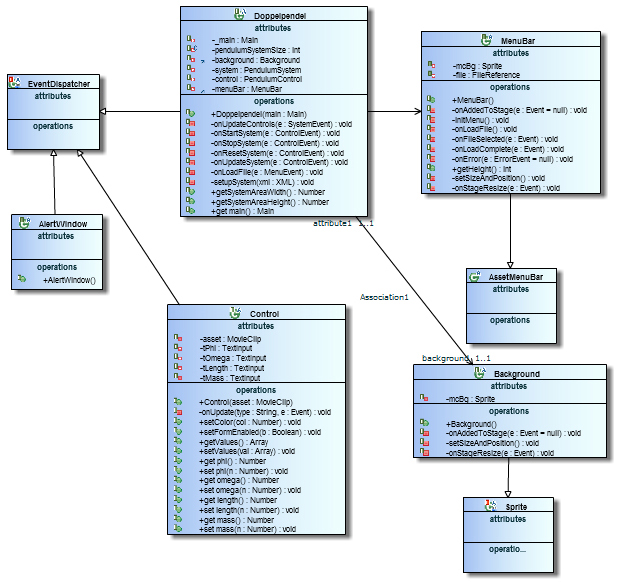
\includegraphics[width=\textwidth]{diag_Doppelpendel.jpg}
	\caption{Klassendiagramm Doppelpendel}
	\label{fig:diag:doppelpendel}
\end{figure}

\begin{figure}[H]
	\centering
	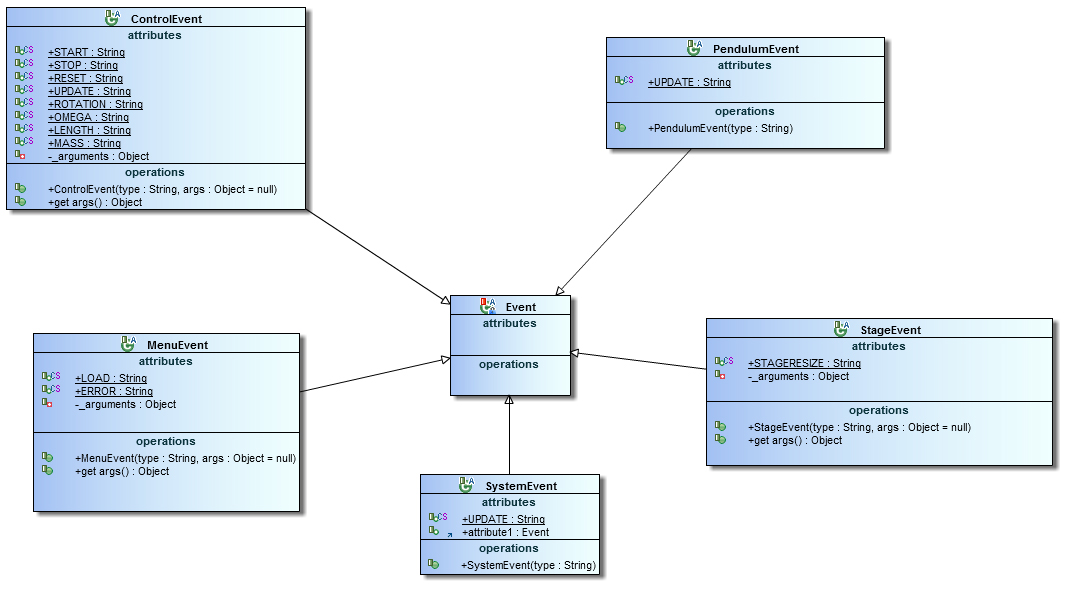
\includegraphics[width=\textwidth]{diag_Event.jpg}
	\caption{Klassendiagramm Eventsystem}
	\label{fig:diag:event}
\end{figure}

\subsubsection{View}
Die View verteilt sich auf die jeweiligen GUI-Klassen \textit{Pendulum}, \textit{PendulumControls}, \textit{Background} und \textit{MenuBar}.

\subsection{Solver Klassen (Runge-Kutta)}
Die Bewegungsgleichung des Doppelpendels wird in drei abgetrennten Klassen berechnet. Die Klasse \textit{PendulumSystem} nimmt die aktuellen Werte der Pendel entgegen und leitet sie zum Berechnen an die Klassen \textit{RungeKutta} und \textit{PendulumSolver} weiter. Die Klasse \textit{RungeKutta} nähert die Differentialgleichung, die in der Klasse \textit{PendulumSolver} definiert ist, über das RK4-Verfahren an. Die Lösung wird als Vektor im \textit{PendulumSolver} gespeichert.

\begin{figure}[H]
	\centering
	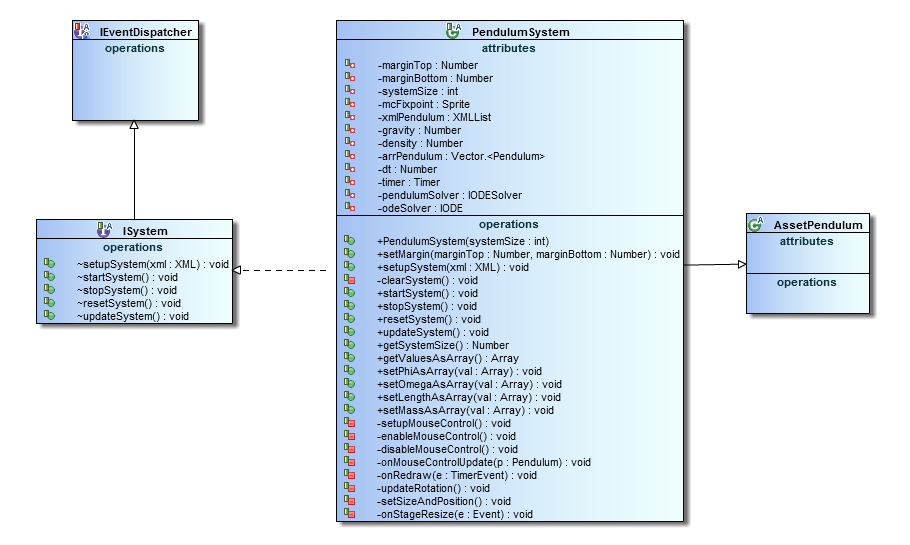
\includegraphics[scale=0.45]{diag_PendulumSystem.jpg}
	\caption{Klassendiagramm Pendulumsystem}
	\label{fig:diag:pendulumSystem}
\end{figure}

\begin{figure}[H]
	\centering
	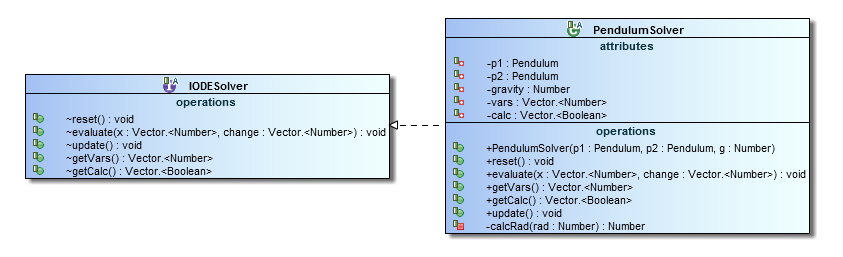
\includegraphics[scale=0.45]{diag_IODESolver.jpg}
	\caption{Klassendiagramm PendulumSolver/IODESolver}
	\label{fig:diag:iodeSolver}

\end{figure}
\begin{figure}[H]
	\centering
	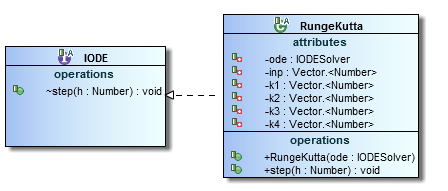
\includegraphics[scale=0.45]{diag_IODE.jpg}
	\caption{Klassendiagramm RungeKutta/IODE}
	\label{fig:diag:iode}
\end{figure}

\subsection{Konfiguration des Systems}
\subsubsection{Konfigurationsdateien}
Die Software arbeitet mittels Konfigurationsdateien, um die verschiedenen Anfangswerte eines Doppelpendels laden zu können. Die Konfigurationsdateien sind im XML Format definiert. Es wird für die Dateien eine eigene Dateiendung verwendet. Die IDP-Datei (IDP steht für Inverses Doppel Pendel) kann in jedem Texteditor bearbeitet werden.

Beispiel einer IDP-Konfigurationsdatei:
\begin{figure}[H]
	\centering
	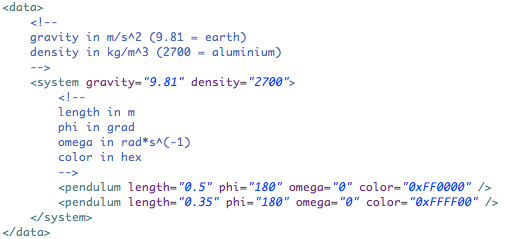
\includegraphics[width=\textwidth]{xml.png}
	\caption{IDP Konfigurationsdatei}
	\label{fig:xml}
\end{figure}

% Fazit
\newpage
\section{Fazit Projektarbeit}
Die Entscheidung die Projektarbeit mit AS3 und dem FlexSDK zu entwickeln, erwies sich schnell als richtig. Die grundlegenden Strukturen der Applikation konnten in kurzer Zeit umgesetzt werden und dem Experten zur Ansicht vorgelegt werden. Um den Effekt der Pendelbewegung  möglichst schnell zu visualisieren, wurde die Bewegung zu beginn als lineare Animation implementiert. Die Animation der Pendel konnte dank der losen Kopplung der AS3 Strukturen leicht gegen die finale Bewegungsgleichung ausgetauscht werden.

Obschon wir mit dem Resultat der Implementierung in AS3 sehr zufrieden sind, mussten wir feststellen, dass die AS3 Programmiersprache bezüglich Performance von Realtime Berechnungen gewisse Nachteile mit sich brachte. Die Animation des Doppelpendels ruckelte zu Beginn relativ Stark, was uns zu umfangreichen Optimierungen im Renderer des Pendelsystems gezwungen hat.

Die Projektarbeit über das Doppelt inverse Pendel ermöglichte uns wertvolle Einblicke in physikalische Problemstellungen und deren numerische Lösungsverfahren. Insgesamt war diese Projektarbeit für uns sehr spannend und aufschlussreich.

\newpage
\listoffigures

\newpage
\nocite{*}
\bibliographystyle{plainnat}
\bibliography{books}

\appendix
\section{Projektplan}
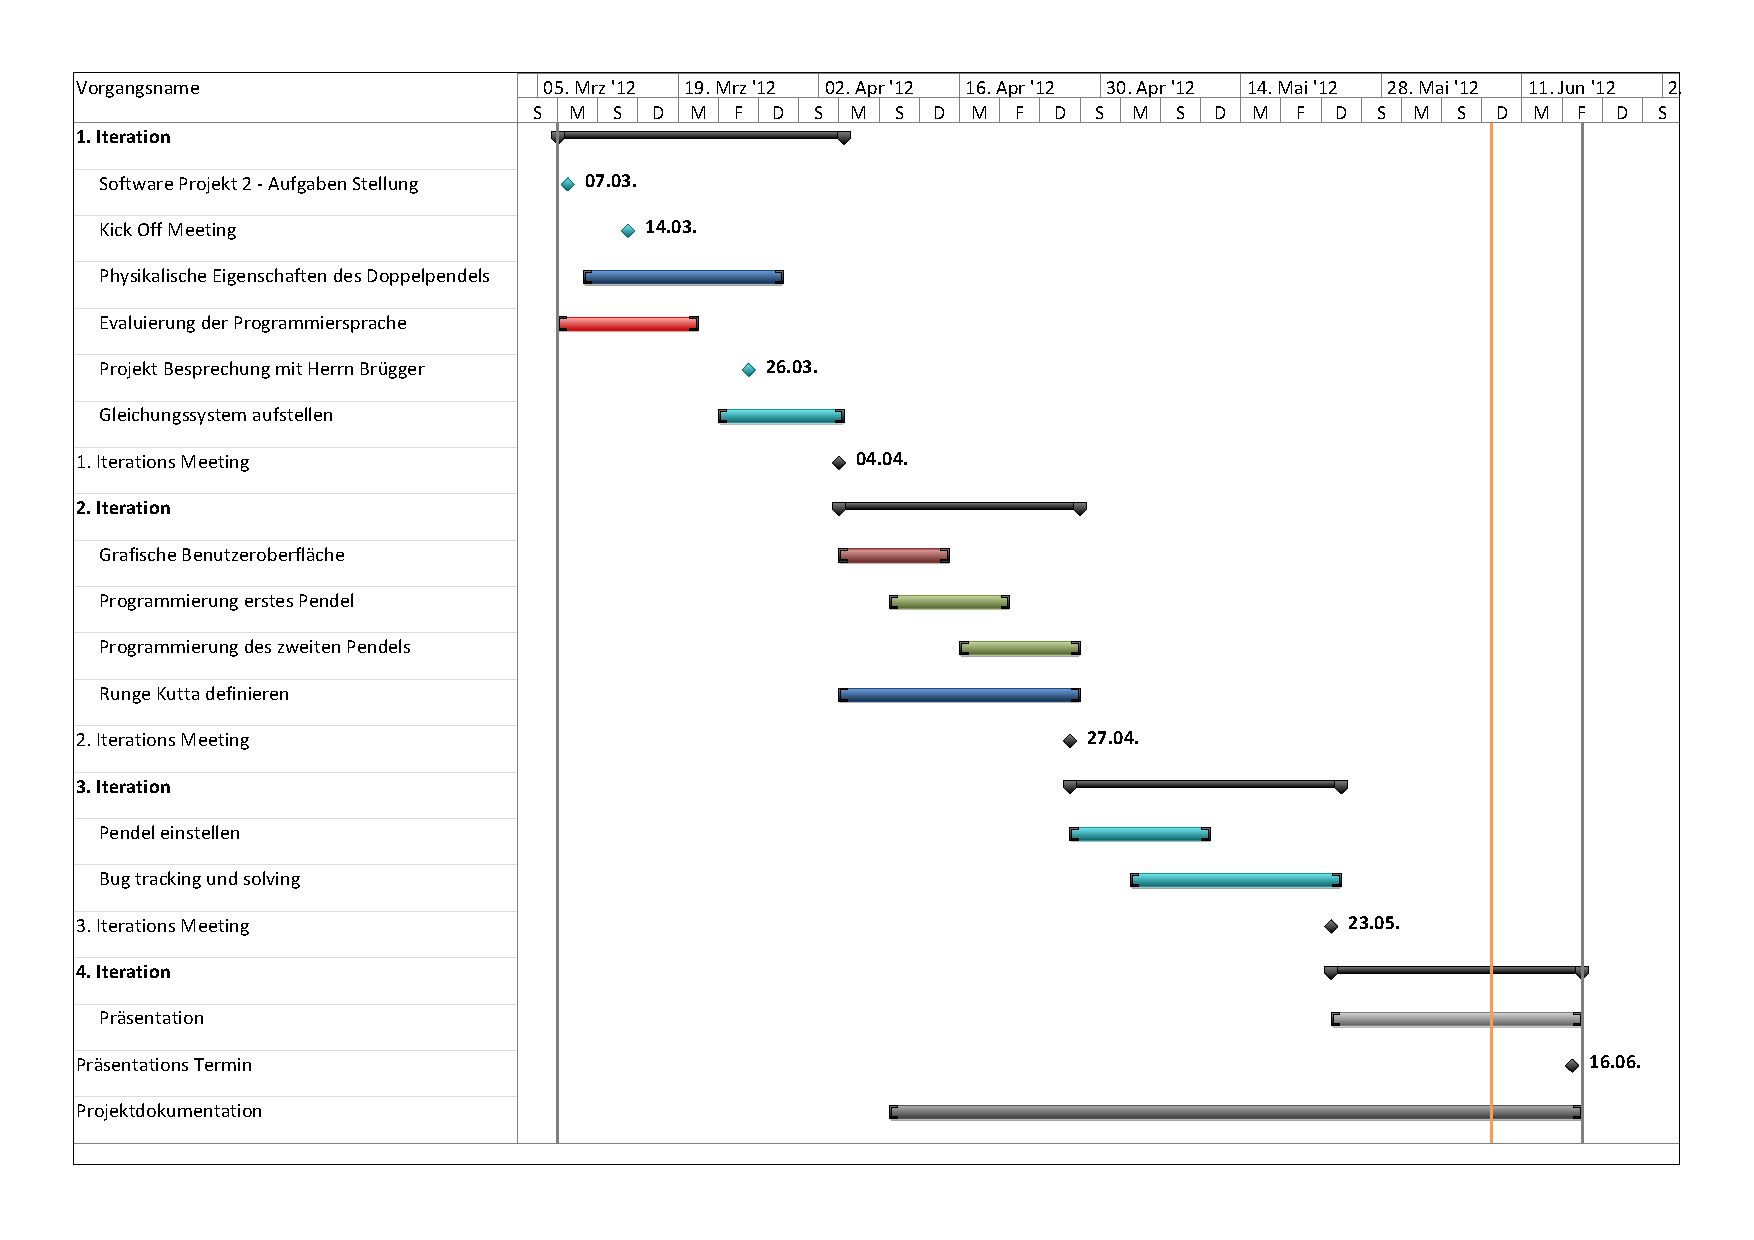
\includegraphics[angle=90, width=\textwidth]{projektplan.pdf}

\end{document}  